\subsection{Pythonic Idioms}
\label{idioms}
Using the sampling approach described in section~\ref{sampling}, we sampled 25 most popular Python idioms from work of Alexandru et al.~\cite{Alexandru2018} and Farook et al.~\cite{idioms}. 
We then compared Copilot suggestions when prompted with an input~(shown in section~\ref{input}) to trigger a code suggestion from Copilot and present our results using the evaluation approach~(shown in section~\ref{evaluation}).

Copilot suggested the idiomatic approach as the first suggestion in 2 of the 25 idioms we tested i.e., 2 out of 25 instances Copilot had the recommended idiomatic approach as its top suggestion. 
However, 8 out of those remaining 23 Idioms had the idiomatic way in Copilot's top 10 suggestions. Copilot did not have the idiomatic way in any of its top 10 suggestions for 15 idioms out of 25 idioms we tested.

The results show that Copilot did not suggest the optimal way as its first suggestion in the majority~(92\%) of the idioms we tested. This shows that current \cct{} like Copilot cannot suggest the idiomatic way even though they are the top most frequently used Python idioms in public repositories on GitHub~\cite{Alexandru2018, idioms}. 

Copilot being closed source we cannot investigate the potential reasons behind this behavior. However, one plausible explanation for this behavior is that idiomatic ways may not be as frequent as non-idiomatic ways in Copilot's training data of public repositories on GitHub, making the non-idiomatic way rank higher than the idiomatic way.

\begin{figure}[hbt!]
    \centering
    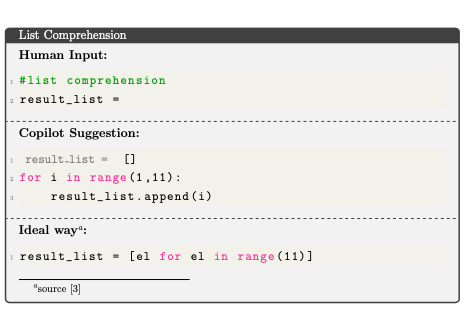
\includegraphics[width=\linewidth]{Figures/idioms_1.png}
    \caption{List Comprehension Idiom and Copilot Suggestion}
    \label{fig:idioms_1}
\end{figure}

Figure~\ref{fig:idioms_1} shows the example of list comprehension Pythonic idiom, showing user input (i.e., human input), the top suggestion by Copilot and the idiomatic way from Alexandru et al.~\cite{Alexandru2018}.

\cct{} like Copilot should learn to detect idiomatic ways in public repositories and rank them higher than the most frequently used way in public repositories, so that the first suggestion would be the idiomatic way rather than the non-idiomatic way, which is the desirable behavior for \cct{} like Copilot. For the scope of this thesis, we leave resolving this problem as future work.

% \begin{tcolorbox}[title=List Comprehension,boxsep=.25mm]
%     %https://tex.stackexchange.com/questions/337909/tcolorbox-tcbline-style
% \textbf{Human Input:}
% \begin{lstlisting}[language={Python}]
% #list comprehension
% result_list = 
% \end{lstlisting}
% \tcbline
% \textbf{Copilot Suggestion:}
% \begin{lstlisting}[language=Python,escapechar=\%]
% % \noindent\textcolor{gray}{result\_list  =} % []
% for i in range(1,11):
%     result_list.append(i)
% \end{lstlisting}
% \tcbline
% \textbf{Idiomatic way\footnote{source \cite{Alexandru2018}}:}
% \begin{lstlisting}[language=Python]
% result_list = [el for el in range(11)]
% \end{lstlisting}
% \end{tcolorbox}

%%%%%% TODO: remember to update the screenshot if the source citation is different from the citation in the text %%%%%%
Table~\ref{tab:all_idioms} shows the list of all the 25 idioms we tested and the ranking of the idiomatic way in Copilot suggestions (if it exists).
All the Idioms shown in Table~\ref{tab:all_idioms} can be found in the \repl{} including the code used as input (i.e., human input), the top suggestion by Copilot and the idiomatic way suggested in Alexandru et al.~\cite{Alexandru2018} and Farook et al.~\cite{idioms}. 

\renewcommand{\arraystretch}{1.45}
\begin{table}[hbt!]

    \begin{tabular}{|c|c|c|}
        \hline
        \centering
         \textbf{S No.} & \textbf{Idiom Title} & \textbf{Copilot Suggestion Matched?}  \\
         & & (out of 10 suggestions) \\
         \hline
         1 & List comprehension & No \\
         \hline
         2 & Dictionary comprehension & No \\
         \hline
         3 & Mapping & 9\textsuperscript{th} \\
         \hline
         4 & Filter &  7\textsuperscript{th} \\
         \hline
         5 & Reduce & 9\textsuperscript{th} \\
         \hline
         6 & List enumeration & No \\
         \hline
         7 & Set comprehension & 1\textsuperscript{th} \\
         \hline
         8 & Read and print from a file & 5\textsuperscript{th} \\
         \hline
         9 & Add int to all list numbers & No \\
         \hline
         10 & If condition check value & 1\textsuperscript{th} \\
         \hline
         11 & Unpacking operators & No \\
         \hline
         12 & Open and write to a file & 6\textsuperscript{th} \\
         \hline
         13 & Access key in dictionary & No \\
         \hline
         14 & Print variables in strings & No \\
         \hline
         15 & Index of every word in input string & No \\
         \hline
         16 & Boolean comparision & 2\textsuperscript{nd} \\
         \hline
         17 & Check for null string & 5\textsuperscript{th} \\
         \hline
         18 & Check for empty list & 4\textsuperscript{th} \\
         \hline
         19 & Multiple conditions in if statement & No \\
         \hline
         20 & Print everything in list & No \\
         \hline
         21 & Zip two lists together & No \\
         \hline
         22 & Combine iterable separated by string & No \\
         \hline
         23 & Sum of list elements & No \\
         \hline
         24 & List iterable creation & No \\
         \hline
         25 & Function to manage file & No \\
         \hline
    \end{tabular}
    \caption{List of all Pythonic idioms tested on Copilot.}
    \label{tab:all_idioms}
\end{table}